\section{Confidence Ellipses}
Let the estimate $(\hat{X_1},\hat{X_2})$ represent the coordinates of one particular network point. These estimated coordinates have the covariance matrix
\begin{equation}
\Sigma=
\begin{bmatrix}
\sigma^2_1 & \sigma_{12}\\
\sigma_{21} & \sigma^2_2
\end{bmatrix}
=\sigma^2_0
\begin{bmatrix}
s^2_1 & s_{12}\\
s_{21} & s^2_2
\end{bmatrix}
=\sigma^2_0Q.
\end{equation}

\begin{table}
Table 4.7\; The important formulas for weighted least squares
\centering
\begin{tabular}{c c}
	\hline 
	Observation equations (A is m by n)& Ax = b-e \\ 
	Covariance matrix for observations&  $\Sigma_b(notice\,\sigma^2_0=1\,a\,priori)$  \\
	Weight matrix (m by m)&   $C=\Sigma^{-1}_b$\\
	Normal equations (n by n)&  $A^TCA\hat{x}=A^TCb$ \\
	Solution of normal equations&   $\hat{x}=(A^TCA)^{-1}A^TCb$\\
	Estimated observations&   $\hat{p}=A\hat{x}=A(A^TCA)^{-1}A^TCb$\\
	Estimated residuals &   $\hat{e}=b-\hat{p}=b-A\hat{x}$\\
	Estimated weighted sum of squares &   $\hat{e}^TC\hat{e}=b^TCb-b^TCA\hat{x}$\\
	Estimated variance of unit weight&  $\hat{\sigma}^2_0=\hat{e}^TC\hat{e}/(m-n)$\\
	Covariance matrix P for unknowns &   $\Sigma_{\hat{x}}=\hat{\sigma}^2_0(A^TCA)^{-1}=(A^T\Sigma^{-1}_bA)^{-1}$\\
	Covariance matrix for observations& $\Sigma_{A\hat{x}}=\hat{\sigma}^2_0(A^TCA)^{-1}A^T$  \\ 
	Covariance matrix for residuals& $\Sigma_{\hat{e}}=\hat{\sigma}^2_0(C^{-1}-A(A^TCA)^{-1}A^T)$\\  
	\hline 
\end{tabular} 	
\end{table}
This 2 by 2 matrix is positive definite; so its inverse exists and is likewise positive definite.
We introduce a local coordinate system with origin at $(\hat{X_1},\hat{X_2})$ and with axes parallel to the original ones. A statistician would write $x~N_2(0,\sigma^2_0Q)$ which means that $(x_1,x_2)$ has a two-dimensional normal distribution with mean (0,0) and covariance matrix$\sigma^2_0Q$.

In the local system $(x_1,x_2)$ is a point on the curve described by the quadratic form
\begin{equation}
x^T\Sigma^{-1}x=c^2.
\end{equation}
This curve is an ellipse because $\Sigma^{-1}$ is positive definite. It is the confidence ellipse of the point — or error ellipse if it is conceived as a pure geometric quantity. It corresponds to the M - file errell.

We denote a unit vector in the direction $\varphi$ by $\xi=(cos\varphi,sin\varphi)$. The expression
\begin{equation*}
\xi^T=cos\varphi x_1+sin\varphi x_2.
\end{equation*}
is the point error in the direction of $\xi$. It is the projection of x in this direction$\xi$.

From the law $B\Sigma_xB^T$ of error propagation in (4.71), the variance of $\xi^T=Bx$ is
\begin{equation}
\sigma^2=\xi^T\Sigma_{\xi}=\sigma^2_1cos^2_{\varphi}+2\sigma_{12}cos\varphi sin\varphi+\sigma^2_2sin^2_{\varphi}.
\end{equation}
The maximum and minimum values are in the directions of the axes of the confidence
ellipse (eigenvectors of $\Sigma$). They are found as solutions to the equation $d\sigma^2/d\varphi=0$:
\begin{equation*}
-(\sigma^2_1-\sigma^2_2)sin2\varphi+2\sigma_{12}cos2\varphi=0.
\end{equation*} 
If $\sigma^2_1=\sigma^2_2$ then the ellipse is oriented in the direction $\varphi=45^{\circ}$. If furthermore $\sigma_{12}=0$ then the axes are indeterminate and $\Sigma=\sigma^2I$ and the ellipse is a circle. In all other cases the direction $\varphi$ of the eigenvector axis is determined through
\begin{equation}
tan2\varphi=\frac{2\sigma_{12}}{\sigma^2_1-\sigma^2_2}.
\end{equation}

\begin{figure}[h]
	\centering
	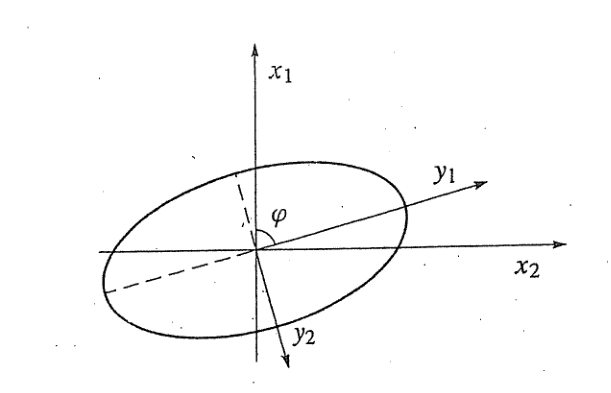
\includegraphics[width=0.7\linewidth]{TeX_files/Part02/chapter04/image/4-10}
	\caption{Figure 4.10\;The principal axes of the confidence ellipse $x^T\Sigma^{-1}x=c^2$}
	\label{fig:4-10}
\end{figure}

Now we rotate the $x_1x_2$ system by this angle$\varphi$ around the point $(\hat{X_1},\hat{X_2})$ to a $y_1y_2$ system. The $y_1$ axis is collinear with the major axis of the confidence ellipse; the off-diagonal entries of the covariance matrix now vanish; hence $y_1$ and $y_2$ are independent. The eigenvectors of $\Sigma$ are diagonalizing the matrix (and its inverse). Since$y_1$ is in the direction of the major axis we have $\lambda_1>\lambda_2$ and the equation of the ellipse is
\begin{equation}
[y_1\;y_2]
\begin{bmatrix}
\lambda_1 & 0\\
0 & \lambda_2
\end{bmatrix}^{-1}
\begin{bmatrix}
y_1 \\y_2
\end{bmatrix}
=c_2.
\end{equation}
or
\begin{equation}
\frac{y^2_1}{(c\sqrt{\lambda_1})^2}+\frac{y^2_2}{(c\sqrt{\lambda_2})^2}=1.
\end{equation}
Notice that $\lambda_1$ and $\lambda_2$ are the eigenvalues $\Sigma$. They are given by
\begin{equation}
\left.
\begin{array}{c c}
\lambda_1 \\ \lambda_2
\end{array}
\right\rbrace
=\frac{1}{2}(\sigma^2_1+\sigma^2_2\pm \sqrt{(\sigma^2_1+\sigma^2_2)^2-4(\sigma^2_1-^2_2-\sigma^2_{12})}).
\end{equation}
By this we have the explicit expressions for determining the confidence ellipse:

1\;The semi major axis is $a=c\sqrt{\lambda_1}$

2\;The semi minor axis is $b=c\sqrt{\lambda_2}$

3\;The major axis is rotated by the angle $\varphi$ away from the $x_1$ axis. 

	\subsection{The Support Function}
	The confidence ellipse is fully described. For completeness, we shall demonstrate a geometric interpretation of the variance $\sigma^2$ in (4.89) in the direction For convenience we rotate the ellipse to the $y_1y_2$ principal axes, and use $\psi$ for the angle from the $y_1$ axis. The equation of the ellipse is
	\begin{equation}
	\frac{y^2_1}{a^2}+\frac{y^2_2}{b^2}=1.
	\end{equation}
	The support function $p(\psi)$ is the maximum of $y_1cos\psi+y_2sin\psi$ over the ellipse: the
	projection of the ellipse in direction $\psi$. This is not the distance from (0,0) to the boundary along the $\psi-line$. If the tangent perpendicular to that direction touches the ellipse at $y_\psi$, then the support $p(\psi)$ measures the projection of $y_\psi$ in the direction $\psi$.
	
	Figure 4.11 shows the support distance p(0), measured to the vertical tangent perpendicular to $\psi=0$. It also shows the distance $p(\frac{\pi}{2})$ to the horizontal tangent. All convex
	sets have support functions p. For an ellipse this is a fourth-order curve and not easily
	drawable, see Figure 4.11. The M-file support calculates and plots the support function of
	any ellipse, given the positive definite matrix $\Sigma$.
	
	Confidence ellipses close to circular shape are close to their support curves. But for
	flat ellipses the difference is large except in the four small sectors around the end points.
	
	We can connect $p(\psi)$ to $\sigma$ in (4.89). The length of the projection of the tangent
	point $y_\psi=(y_1,y_2)$ is
	\begin{equation*}
	p(\psi)=|y_1cos\psi+y_2sin\psi|.
	\end{equation*}
	We square this expression and get
	\begin{equation}
	p^2(\psi)=y^2_1cos^2_\psi+2y_1y_2cos\psi sin\psi+y^2_2sin^2\psi.
	\end{equation}
	The equation for the tangent to the ellipse at $y_\psi$is
	\begin{equation*}
	-\frac{y_1}{a^2}sin\psi+-\frac{y_2}{b^2}cos\psi=0.
	\end{equation*}
	We square and multiply by $a^2b^2$:
	\begin{equation*}
	\frac{b^2y^2_1}{a^2}sin^2_\psi+\frac{a^2y^2_2}{b_2}cos^2_\psi-2y_1y_2sin\psi cos\psi=0.
	\end{equation*}
	Next we add this to (4.95) in order that the mixed products cancel:
	\begin{equation*}
	\begin{split}
	p^2(\psi)&=(y^2_1cos^2_\psi+\frac{b^2}{a^2}y^2_1sin^2_\psi)+(y^2_2sin^2\psi+\frac{a^2}{b_2}y^2_2cos^2_\psi)\\
	&=(\frac{y^2_1}{a^2}+\frac{y^2_2}{b^2})(a^2cos^2_\psi + b^2sin^2_\psi).
	\end{split}
	\end{equation*} 
	Using (4.94) for the special point $y_\psi$ we get
	\begin{equation*}
	p^2(\psi)=a^2cos^2_\psi + b^2sin^2_\psi=[cos\psi\;sin\psi]\begin{bmatrix}
	c^2\lambda_1 & 0\\ 0&c^2\lambda_2
	\end{bmatrix}
	\begin{bmatrix}
	cos\psi \\ sin\psi
	\end{bmatrix}.
	\end{equation*}
	In the original $x_1x_2$ system (where the angle is $\psi$) this is
	\begin{equation}
	p^2(\psi)=[cos\psi\;sin\psi]
	\begin{bmatrix}
	\sigma^2_1 & \sigma_{12}\\ \sigma_{12} & \sigma^2_2
	\end{bmatrix}
	\begin{bmatrix}
	cos\psi \\ sin\psi
	\end{bmatrix}.
	\end{equation}
	This proves that the support function is actually the standard deviation $\sigma$ in (4.89).
	
	\begin{figure}[h]
		\centering
		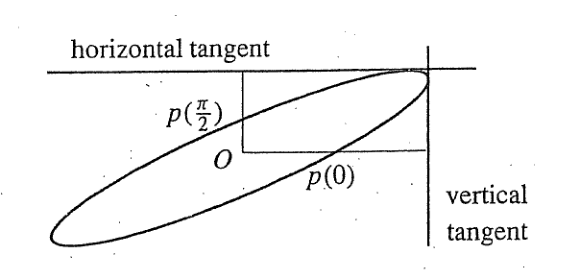
\includegraphics[width=0.7\linewidth]{TeX_files/Part02/chapter04/image/4-11}
		\caption{}
		\label{fig:4-11}
	\end{figure}
	Figure 4.11\; The support function p at $\varphi=0$ and $\varphi=\pi/2$: ellipse for $\Sigma=\begin{bmatrix}
	2 & -4 \\ -4 & 10 \end{bmatrix}$
	
	The preceding considerations were all based on a geometrical view of the quadratic form
	$x^T\Sigma^{-1}x=constant$. This view shall now be complemented by a statistical aspect.
	
	The degree of confidence $\alpha$ for the ellipse (4.88) is given by the probability that
	the ellipse contains the true position $(X_1,X_2)$. There are two situations: the covariance
	matrix $\Sigma$ can be known or it may need rescaling by an unknown factor. Either $\sigma^2_0$ or else the variance is estimated by $\hat{\sigma}^2_0=r^T\Sigma^{-1}r/(m-n)$.
	
	Known covariance matrix The random variables $y_1/c_\alpha\sqrt{\lambda_1}$ and $y_2/c_\alpha\sqrt{\lambda_2}$ are independent and normally distributed with mean value 0 and variance 1. The constant c in (4.88) can be associated with a given probability $\alpha$. In that case we use $c_\alpha$. Statistics tells us that the sum of squares $(y_1/c_\alpha\sqrt{\lambda_1})^2+(y_2/c_\alpha\sqrt{\lambda_2})^2$ is $\chi^2-distributed$ with 2 degrees of freedom. The probability that
	\begin{equation}
	\frac{y^2_1}{(c_\alpha \sqrt{\lambda_1})^2}+\frac{y^2_2}{(c_\alpha \sqrt{\lambda_2})^2}\leq 1
	\end{equation}
	is $K(c^2_\alpha)=1-e^{-c^2_\alpha/2}$,cf.(4.50) and Table 4.3. Specifically this means that if the confidence ellipse is a circle with radius 10 cm, then every 10th sample point falls outside a circle with radius 21.5cm. Every 20th point falls outside a circle with radius 24.5cm.
	
	Unknown covariance matrix We insert (4.87) into the quadratic form (4.88) and get 
	\begin{equation}
	x^T\Sigma^{-1}x=\frac{x^TQ^{-1}x}{\hat{\sigma}^2_0}.
	\end{equation}
	The numerator and denominator are independent with the distributions for $\chi^2_2$ and
	$\chi^2_{m-n}$. Hence the left side has the $F_{2,m-n}$ distribution given by (4.51). Note that Q is known a
	priori.
	
	For m - n sufficiently large, say 50, we can act as if $\hat{\sigma}^2_0$ were known; see Abramowitz \& Stegun (1972), Table 26.9. Choose $\alpha$ and $c^2_\alpha$ such that for the F distribution,
	\begin{equation*}
	Prob(x^T\Sigma^{-1}x/2\leq c^2_\alpha)=Prob(F_{2,m-n}\leq c^2_\alpha)=\alpha.
	\end{equation*} 
	This describes the ellipse in which x must lie with the prescribed probability $\alpha$.
	
	\begin{figure}[h]
		\centering
		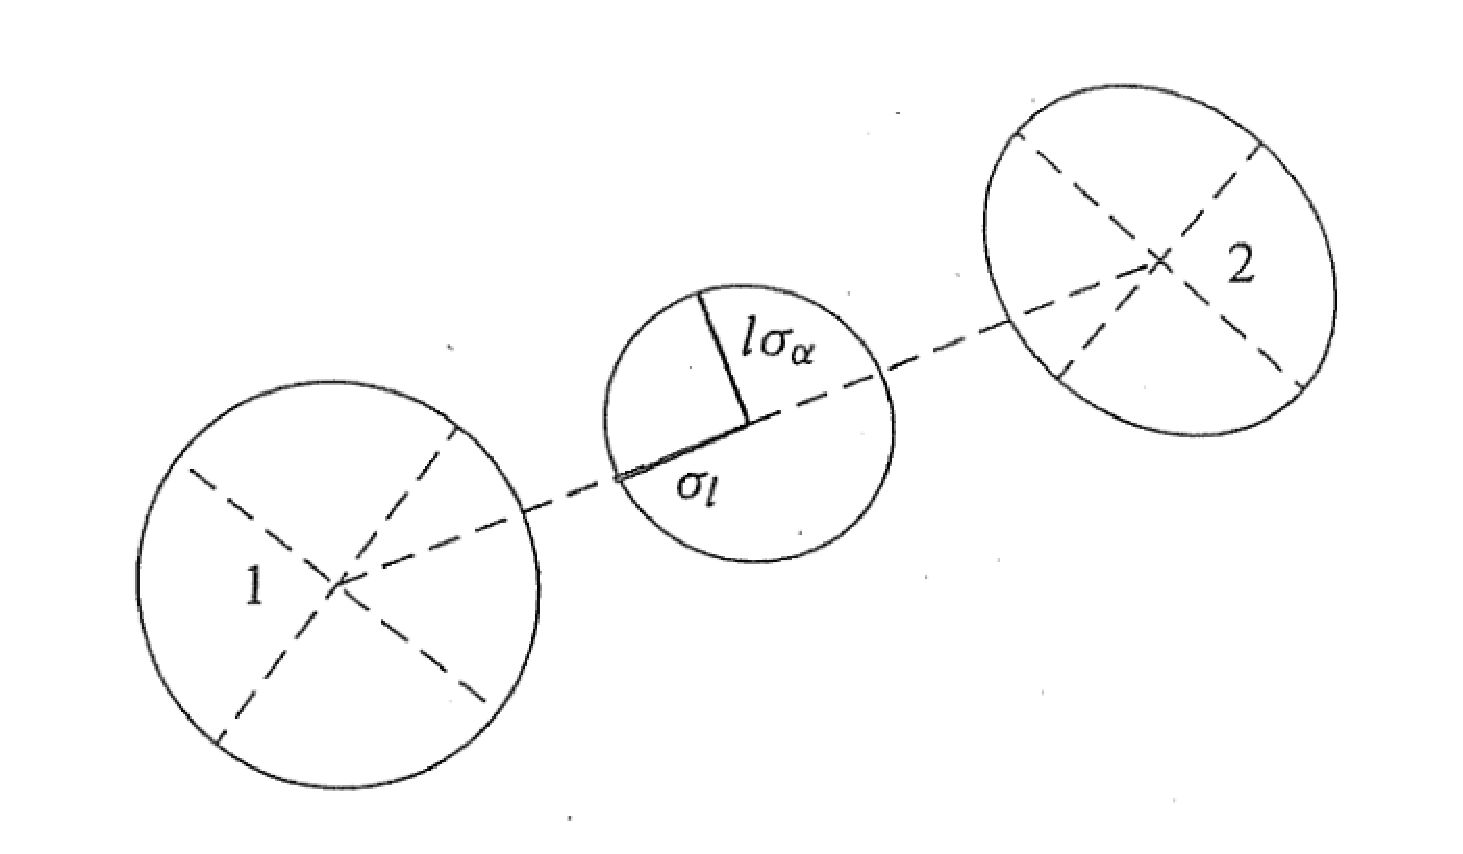
\includegraphics[width=0.7\linewidth]{TeX_files/Part02/chapter04/image/4-12}
		\caption{Figure 4.12\; Confidence ellipses of points 1 and 2 and their relative confidence ellipse.}
		\label{fig:4-12}
	\end{figure}	
	The figure illustrates the geometrical meaning of $\sigma_l$ and $\sigma_\alpha$ as defined in (4.87).
	
	\subsection{Relative Confidence Ellipses}
	A very important step in geodesy and GPS is to work with differences. We saw a one-dimensional example in Section 4.4 and in the M-file oned. The separate errors from a satellite to two receivers partly disappeared in the difference $x_2-x_1$. The large tilted error
	ellipse (with off-diagonal correlation from the shared satellite error) became a smaller up-right ellipse in Figure 4.9 from a diagonal covariance matrix. This is the relative confidence ellipse. We now extend this idea to two dimensions.
	
	Points 1 and 2 have coordinates $(x_1,y_1)$ and $(x_2,y_2)$. The vector d between the
	points has components
	\begin{equation*}
	dx=x_2-x_1  \quad and \quad dy=y_2-y_1.
	\end{equation*}
	This vector comes from multiplying the full set of four unknowns $x_1,y_1,x_2,y_2$ by the
	matrix
	\begin{equation*}
	L=\begin{bmatrix}
	-1 & 0 & +1 & 0 \\
	0 & -1 & 0 & +1 
	\end{bmatrix}
	=
	[-I\;I].
	\end{equation*}
	Then the propagation law says that the covariance matrix of the vector $d=(dx,dy)$ is
	$\Sigma_d=L\Sigma L^T$:
	\begin{equation}
	\Sigma_d=[-I\;I]\begin{bmatrix} \Sigma_1 & \Sigma_{12}\\ \Sigma^T_{12} & \Sigma_2
	\end{bmatrix}
	\begin{bmatrix}
	-I \\I
	\end{bmatrix}
	=
	[\Sigma_1-\Sigma_{12}-\Sigma^T_{12}+\Sigma_2].
	\end{equation} 
	Each of these blocks is 2 by 2. The blocks $\Sigma_1$ and $\Sigma_2$ contain covariances for point 1 and point 2 separately.
	
	The off-diagonal blocks $\Sigma_{12}$ and $\Sigma^T_{12}$ in the full 4 by 4 symmetric matrix $\Sigma$ contain covariances $\sigma_{x_1x_2},\sigma_{x_1y_2},\sigma_{x_2y_1},\sigma_{x_2y_2}$, between points 1 and 2. Then the combination (4.99) of the four blocks is the relative covariance matrix $\Sigma_d$:
	\begin{equation}
	\Sigma_d=
	\begin{bmatrix}
	\sigma^2_{x_1}-2\sigma_{x_1x_2}+\sigma^2_{x_2} & \sigma_{x_1y_1}-\sigma_{x_1y_2}-\sigma_{x_2y_1}+\sigma_{x_2y_2}\\
	\sigma_{x_1y_1}-\sigma_{x_1y_2}-\sigma_{x_2y_1}+\sigma_{x_2y_2} &
	\sigma^2_{y_1}-2\sigma_{y_1y_2}+\sigma^2_{y_2}
	\end{bmatrix}.
	\end{equation}
	This covariance matrix $\Sigma_d$ produces a relative confidence ellipse with the following 
	remarkable and simple properties. The standard deviation $\sigma_l$ of the length of the vector,
	$l^2=(dx)^2+(dy)^2$, can be found in Figure 4.12. The angle $\alpha$ has tangent dy/dx. The
	quantities $\sigma_l$ and $l\sigma_\alpha$ are determined by the support function in the vector direction and the perpendicular direction. This geometrical construction makes the relative confidence ellipse useful. Of course points 1 and 2 can be any two points in the network.
	
	The relative ellipse is often smaller than the separate ellipses 1 and 2. Typically this
	is the case when the covariances $\sigma_{x_1x_2}$ and $\sigma_{y_1y_2}$ are positive. Then errors common to the two points are removed in their difference $d=(x_2-x_1,y_2-y_1)$.
	
	The M-files relellip and ellaxes compute the relative confidence ellipse.
	
	 